% Template for Elsevier CRC journal article
% version 1.1 dated 16 March 2010

% This file (c) 2010 Elsevier Ltd.  Modifications may be freely made,
% provided the edited file is saved under a different name

% This file contains modifications for Procedia Computer Science
% but may easily be adapted to other journals

% Changes since version 1.0
% - elsarticle class option changed from 1p to 3p (to better reflect CRC layout)

%-----------------------------------------------------------------------------------

%% This template uses the elsarticle.cls document class and the extension package ecrc.sty
%% For full documentation on usage of elsarticle.cls, consult the documentation "elsdoc.pdf"
%% Further resources available at http://www.elsevier.com/latex

%-----------------------------------------------------------------------------------

%%%%%%%%%%%%%%%%%%%%%%%%%%%%%%%%%%%%%%%%%%%%%%
%%%%%%%%%%%%%%%%%%%%%%%%%%%%%%%%%%%%%%%%%%%%%%
%%                                          %%
%% Important note on usage                  %%
%% -----------------------                  %%
%% This file must be compiled with PDFLaTeX %%
%% Using standard LaTeX will not work!      %%
%%                                          %%
%%%%%%%%%%%%%%%%%%%%%%%%%%%%%%%%%%%%%%%%%%%%%%
%%%%%%%%%%%%%%%%%%%%%%%%%%%%%%%%%%%%%%%%%%%%%%

%% The '3p' and 'times' class options of elsarticle are used for Elsevier CRC
\documentclass[3p,times]{elsarticle}

%% The `ecrc' package must be called to make the CRC functionality available
\usepackage{ecrc}

%% The ecrc package defines commands needed for running heads and logos.
%% For running heads, you can set the journal name, the volume, the starting page and the authors

%% set the volume if you know. Otherwise `00'
\volume{00}

%% set the starting page if not 1
\firstpage{1}

%% Give the name of the journal
\journalname{Systems and Software}

%% Give the author list to appear in the running head
%% Example \runauth{C.V. Radhakrishnan et al.}
\runauth{}

%% The choice of journal logo is determined by the \jid and \jnltitlelogo commands.
%% A user-supplied logo with the name <\jid>logo.pdf will be inserted if present.
%% e.g. if \jid{yspmi} the system will look for a file yspmilogo.pdf
%% Otherwise the content of \jnltitlelogo will be set between horizontal lines as a default logo

%% Give the abbreviation of the Journal.
\jid{procs}

%% Give a short journal name for the dummy logo (if needed)
\jnltitlelogo{Systems and Software}

%% Hereafter the template follows `elsarticle'.
%% For more details see the existing template files elsarticle-template-harv.tex and elsarticle-template-num.tex.

%% Elsevier CRC generally uses a numbered reference style
%% For this, the conventions of elsarticle-template-num.tex should be followed (included below)
%% If using BibTeX, use the style file elsarticle-num.bst

%% End of ecrc-specific commands
%%%%%%%%%%%%%%%%%%%%%%%%%%%%%%%%%%%%%%%%%%%%%%%%%%%%%%%%%%%%%%%%%%%%%%%%%%

%% The amssymb package provides various useful mathematical symbols
\usepackage{amssymb}
%% The amsthm package provides extended theorem environments
%% \usepackage{amsthm}

%% The lineno packages adds line numbers. Start line numbering with
%% \begin{linenumbers}, end it with \end{linenumbers}. Or switch it on
%% for the whole article with \linenumbers after \end{frontmatter}.
%% \usepackage{lineno}

%% natbib.sty is loaded by default. However, natbib options can be
%% provided with \biboptions{...} command. Following options are
%% valid:

%%   round  -  round parentheses are used (default)
%%   square -  square brackets are used   [option]
%%   curly  -  curly braces are used      {option}
%%   angle  -  angle brackets are used    <option>
%%   semicolon  -  multiple citations separated by semi-colon
%%   colon  - same as semicolon, an earlier confusion
%%   comma  -  separated by comma
%%   numbers-  selects numerical citations
%%   super  -  numerical citations as superscripts
%%   sort   -  sorts multiple citations according to order in ref. list
%%   sort&compress   -  like sort, but also compresses numerical citations
%%   compress - compresses without sorting
%%
%% \biboptions{comma,round}

% \biboptions{}

% if you have landscape tables
\usepackage[figuresright]{rotating}

% put your own definitions here:
%   \newcommand{\cZ}{\cal{Z}}
%   \newtheorem{def}{Definition}[section]
%   ...

% add words to TeX's hyphenation exception list
%\hyphenation{author another created financial paper re-commend-ed Post-Script}

% declarations for front matter

% Our Packages (UIoT)
\usepackage{graphicx}
\usepackage{epstopdf}
\usepackage{hyperref}
\usepackage{listings}

\begin{document}

\begin{frontmatter}

%% Title, authors and addresses

%% use the tnoteref command within \title for footnotes;
%% use the tnotetext command for the associated footnote;
%% use the fnref command within \author or \address for footnotes;
%% use the fntext command for the associated footnote;
%% use the corref command within \author for corresponding author footnotes;
%% use the cortext command for the associated footnote;
%% use the ead command for the email address,
%% and the form \ead[url] for the home page:
%%
%% \title{Title\tnoteref{label1}}
%% \tnotetext[label1]{}
%% \author{Name\corref{cor1}\fnref{label2}}
%% \ead{email address}
%% \ead[url]{home page}
%% \fntext[label2]{}
%% \cortext[cor1]{}
%% \address{Address\fnref{label3}}
%% \fntext[label3]{}

\dochead{}
%% Use \dochead if there is an article header, e.g. \dochead{Short communication}

\title{A Holistic IoT User-Friendly Management System}

%% use optional labels to link authors explicitly to addresses:
%% \author[label1,label2]{<author name>}
%% \address[label1]{<address>}
%% \address[label2]{<address>}

\author{Claudio A. S. Wunder, Caio C. M. Silva, Rafael T. S. JR}

\address{}

\begin{abstract}
%% Text of abstract
\end{abstract}

\begin{keyword}
%% keywords here, in the form: keyword \sep keyword

%% MSC codes here, in the form: \MSC code \sep code
%% or \MSC[2008] code \sep code (2000 is the default)

\end{keyword}

\end{frontmatter}

%%
%% Start line numbering here if you want
%%
% \linenumbers

\lstset{
		basicstyle=\small,
        breaklines=true
        keywordstyle=\color{black}\bfseries\underbar,
        identifierstyle=, 
        language=PHP,
        commentstyle=\color{white},
        stringstyle=\ttfamily, 
        showstringspaces=false}

\section{Introduction}
\label{introduction}

\section{Related Concepts} % TODO: Change Title
\label{related_concepts}

\section{Proposal}
\label{proposal}

In this section it is presented the IoT management system approach. 
Figure \ref{fig_system_architecture} presents the proposed architecture.
The system architecture was conceived into five layers, denominated, user experience layer (UXL), 
presentation layer (PL), input interpreter layer (IIL), business logic layer (BLL), and communication layer (CL).

\begin{figure}[!ht]
	\centering
	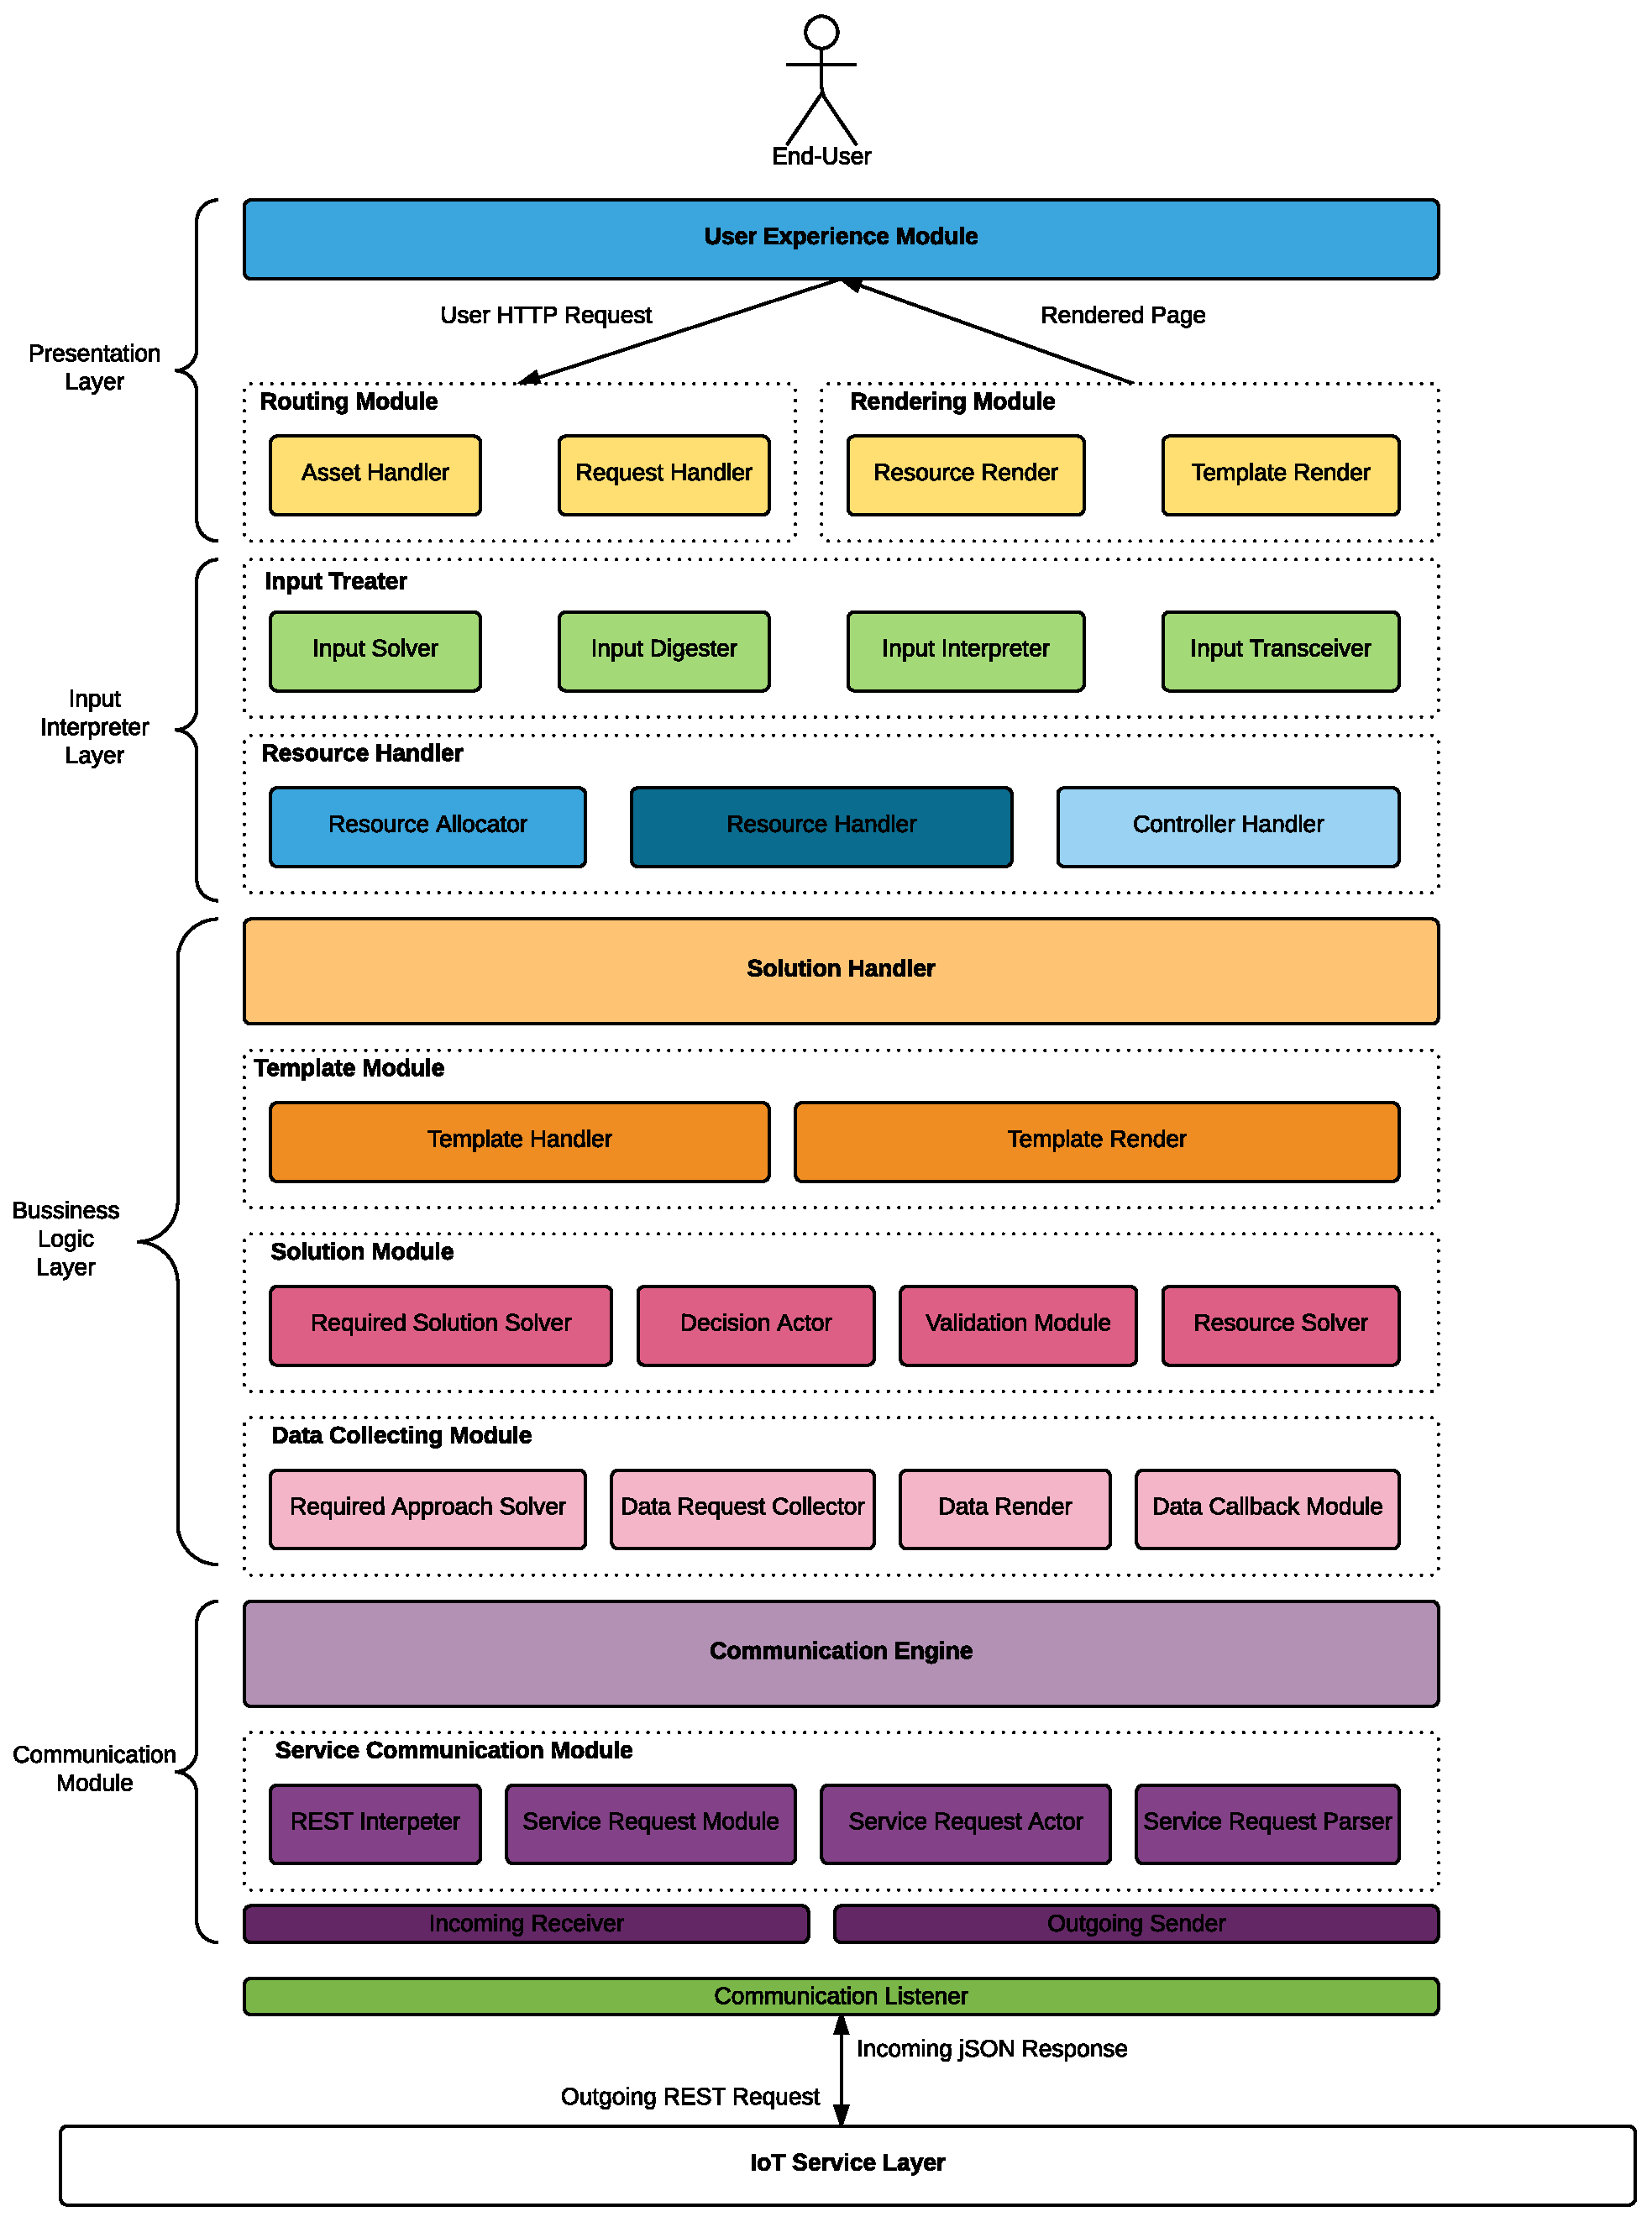
\includegraphics[scale=0.25]{composite_que_quiser.eps}
	\caption{IoT management system architecture.}
	\label{fig_system_architecture}
\end{figure}

Broadly speaking, the UXL was idealized to make possible an IoT management through a natural interface. 
In the other hand, the PL receive a HTTP request, which represents a solicitation of a system
feature, and routes to the respective feature handler. The IIL digest and solve the received data
from PL and invoke the respective system action. The BLL receive the invoked action from IIL and execute the solution
to complete the required feature. The CL does the communication using a REST approach as indicated in \cite{silva2016restiot}, 
sending requests to a service layer.

The proposal presentation is divided into four subsections, where each section describes each architecture layer of
the proposed system. 

\subsection{Presentation Layer}
\label{presentation_layer}

The presentation layer provides a full aware IoT network management context.

\subsubsection{Routing Module}
\label{routing_module}

\subsubsection{Rendering Module}
\label{rendering_module}

\subsection{Input Interpreter Layer}
\label{input_interpreter_layer}

The IIL is liable to understand the requested resource. In order to interpret the submitted request, IIL performs the process presented in Figure \ref{fig_iil_flowchart}.

The figure process starts when PL sends a resource request to IIL. The request data is received by Input Solver which solves and map it.

In the next step, a raw data map is sent to Input Digester, which cleans the data, removing useless and uncomprehensible information. 
If the map does not represent a valid set of information, the data is discarded and the process ends.
In other way, the map is redirect to Input Interpreter which associate the data map elements into valid resource elements. 
Finally, the map is treated in Input Transceiver, joining and associating similar resources. 

Thus, the resource map is routed to Resource Handler Module, which allocate the specific resources into memory.
In addition, the resource handler performs all invocations related to it correspondent resource.

\begin{figure}[!ht]
	\centering
	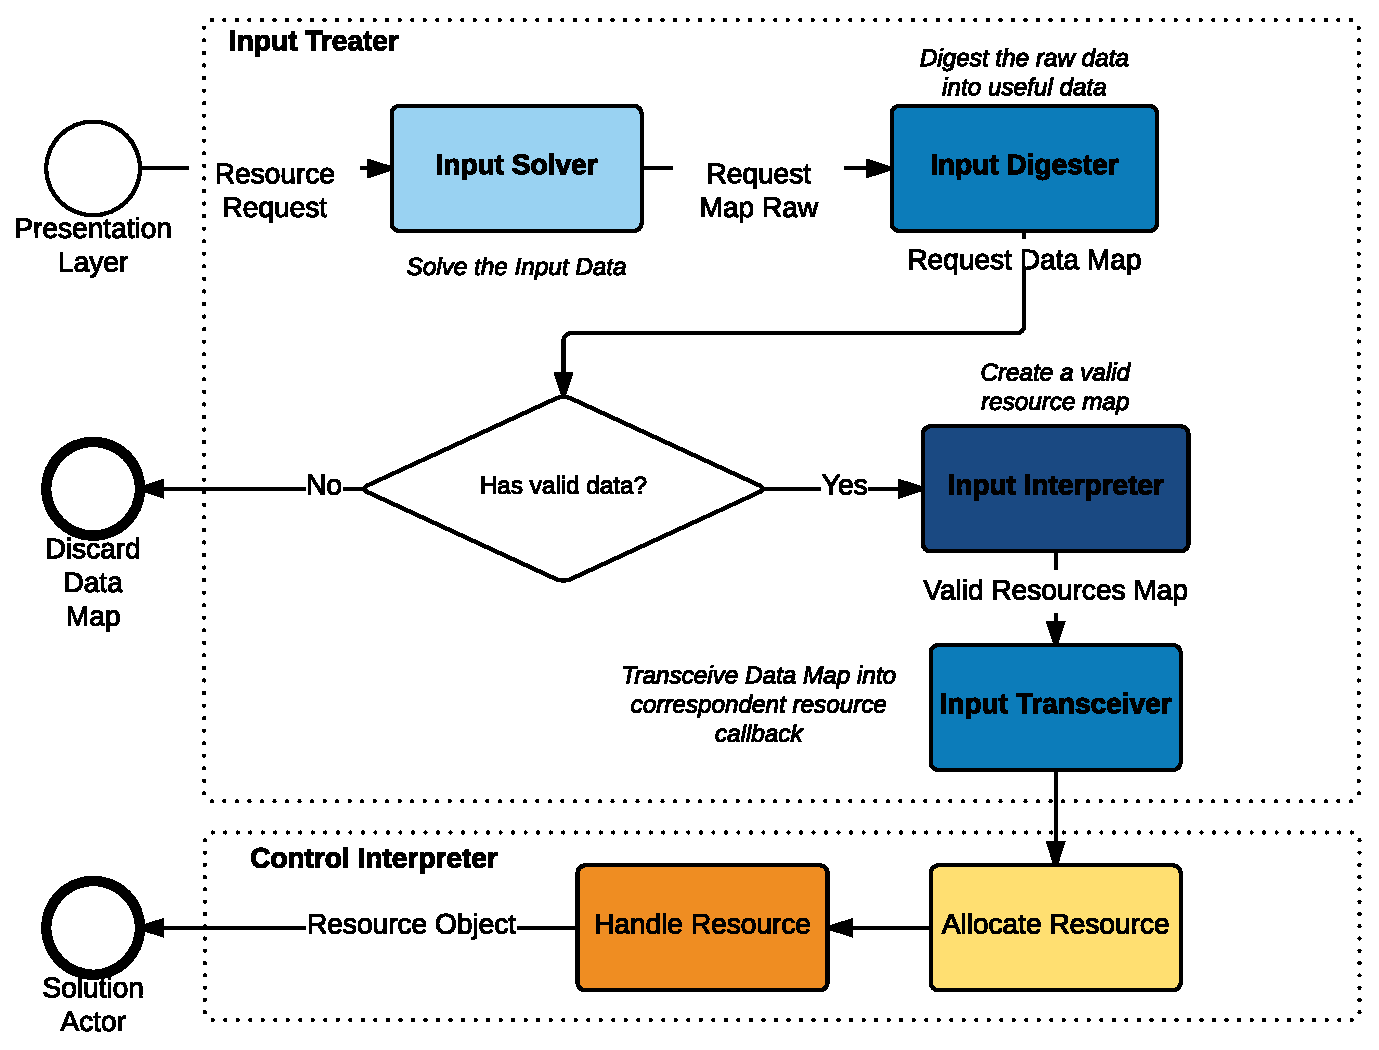
\includegraphics[scale=0.3]{iil_layer.eps}
	\caption{Input Interpreter Layer Flow Chart}
	\label{fig_iil_flowchart}
\end{figure}

The following sub sections intents to explain each component of input interpreter layer, presenting their respective functionalities and limitations.

\subsubsection{Input Treater}
\label{input_treater}

The IT has four components, input solver, input digester, input interpreter and input transceiver.
The input solver and digester use predefined regular expressions to identify which input expressions are valid. 
Those validated expressions are assigned to a correspondent route.

For an example, the Listing \ref{listing_baba} shows a route being created.
The function \textit{addRoute} receives five parameters. The first one indicates
the allowed regular expression for the route. The second one, set the type of node that will be invoked.
Moreover, the third one defines the route segment level. Finally, also is defined the RESTful method, and 
the public route name.

\begin{minipage}{0.475\textwidth}
	\begin{lstlisting}[frame=single, caption=Route Assign, label=listing_baba]
Router::addRoute('/(\w+)', new ActionNode, 2, 'get', 'web_page');
	\end{lstlisting}
\end{minipage}


After the route assign, the input interpreter receives the resource map, which identifies the correspondent resource callback for each data,
ignoring information that does not belong to any existing resource. Thereby, a full comprehensible resource map is obtained, containing valid resource information.
The resource map elements are simplified by input transceiver, which joins resources of the same type.
Finally, the resource map is sent to the resource handling layer, which is explained in Section \ref{resource_handler}.

\subsubsection{Resource Handler}
\label{resource_handler}

\subsection{Business Logic Layer}
\label{business_logic_layer}

\subsubsection{Solution Handler}
\label{solution_handler}

\subsubsection{Template Module}
\label{template_module}

\subsubsection{Solution Module}
\label{solution_module}

\subsubsection{Data Collecting Module}
\label{data_collecting_module}

\subsection{Communication Module}
\label{communication_module}

\subsubsection{Communication Engine}
\label{communication_engine}

\subsubsection{Service Communication Module}
\label{service_communication_module}

% Podem existir subse��es nessa jossa toda, OK?

\subsection{Communication Interface}
\label{communication_interface}

\begin{table}[htb]
	\caption{\label{tabela}\textit{Caption} comes before the table.}
	\begin{center}
		{\tt
			\begin{tabular}{|c||c|c|c|}\hline
				         & title page & odd page  & even page \\\hline\hline
				onesided & leftTEXT   & leftTEXT  & leftTEXT  \\\hline
				twosided & leftTEXT   & rightTEXT & leftTEXT  \\\hline
			\end{tabular}
		}
	\end{center}
\end{table}

\subsection{User Experience} % TODO: Improve it!
\label{ux_layer}

\section{Experimental Environment and Result Analysis}
\label{experimental_tests}

\section{Conclusion and Future Work}
\label{conclusion}

%% The Appendices part is started with the command \appendix;
%% appendix sections are then done as normal sections
%% \appendix

%% \section{}
%% \label{}

%% Acknowledgement
\section*{Acknowledgments}
The authors wish to thank the Brazilian research, development and innovation 
Agencies CAPES (Grant FORTE 23038.007604/2014-69), 
FINEP (Grant RENASIC/PROTO 01.12.0555.00) and the National Post-Doctorate Program (PNPD/CAPES) for their support to this work.

%% References
%%
%% Following citation commands can be used in the body text:
%% Usage of \cite is as follows:
%%   \cite{key}         ==>>  [#]
%%   \cite[chap. 2]{key} ==>> [#, chap. 2]
%%

%% References with BibTeX database:

\bibliographystyle{elsarticle-num}
\bibliography{bibliographyhello}

%% Authors are advised to use a BibTeX database file for their reference list.
%% The provided style file elsarticle-num.bst formats references in the required Procedia style

%% For references without a BibTeX database:

% \begin{thebibliography}{00}

%% \bibitem must have the following form:
%%   \bibitem{key}...
%%

% \bibitem{}

% \end{thebibliography}

\end{document}

